\documentclass[12pt]{article}
\usepackage[backend=biber, style=apa, sorting=none]{biblatex}
\usepackage[margin = 1in]{geometry}
\usepackage{setspace}
\usepackage{paralist}
\usepackage{linguex}
\usepackage{graphicx}
\addbibresource{references.bib}


\begin{document}
\linespread{1.5}
\setstretch{1.5}
\begin{center}
    \thispagestyle{empty}
    \textbf{Application of the AIST LSTM-based Genre Classification Model to the BRACE dataset}

    \vspace{20mm}
    A Special Problem 
    \par Presented to the Faculty of the Division of Physical Sciences and Mathematics 
    \par College of Arts and Sciences 
    \par University of the Philippines Visayas 
    \par
    Miag-ao, Iloilo

    \vspace{20mm}
    By
    \par
    HUPP, James Ezra E.

    \vspace{20mm}
    Ara Abigail Ambita
    \par
    Adviser

\end{center}
\newpage
\tableofcontents
\newpage
\
\section*{Chapter 1}

\section{Introduction}

\subsection{Background and Rationale}
\noindent 
\par Dance embodies a unique category of human activity. With its global prevalence and cultural importance, dance holds a pivotal role in both communal and personal aspects, serving as both a unifying element and an outlet for self-expression. It is composed of several different essences, movements, and poses, all of which fit into a certain dance style, also known as a dance genre. 
\vspace{5mm}

\par In the preceding years, machine learning has emerged as a tool to identify and analyze human activity. Machine learning, which is a branch of Artificial Intelligence (AI), places emphasis on the use of data and algorithms to replicate human learning (IBM, 2019). Furthermore, deep learning is a subset of machine learning which utilizes artificial neural networks consisting of multiple layers (Lgayhardt 2023). With dance being a topic of recent interest, a few datasets have emerged that feature different dance genres, such as AIST \parencite{aist}, Everybody Dance Now \parencite{chan2019everybody}, and BRACE \parencite{brace}. Consequently, some studies have been conducted which have used varying machine learning and deep learning techniques to classify video and audio sequences into their respective dance genres. 
\vspace{5mm}

\par For example, “AIST DANCE VIDEO DATABASE: MULTI-GENRE, MULTI-DANCER, AND MULTI-CAMERA DATABASE FOR DANCE INFORMATION PROCESSING” by \Textcite{aist} applies four baseline methods based on a Support Vector Machine (SVM) based model and a Long Short-Term Memory (LSTM) based model to classify videos from the AIST dataset into one of its 10 dance genres. They found that the LSTM model performed better with 91\% accuracy. It is pertinent to mention that an SVM algorithm is a type of machine learning tool that is used to predict outcomes or categorize items by sorting them into groups \parencite{svm}. Conversely, LSTM  is a type of Recurrent Neural Network that detains long-term dependecies in sequential data \parencite{Banoula_2023} \parencite{sherstinsky2020fundamentals}. Moreover, “Dance Video Classification into Relevant Street Dancing Styles using Deep Learning Techniques” by Bauskar, D. (2022) uses VGG-16 and VGG-19 to perform the same task, also on the AIST dataset. They found that the VGG-16 based model performed best with 75.86\% accuracy. Consisting of 10 dance genres with 13,939 videos \Textcite{aist} and recorded in a controlled setting, AIST provides an ideal dataset for genre classification tasks. However, this raises the question of how current dance genre classification models perform when tested against more complex, unstructured videos.
\vspace{5mm}

\par The BRACE dataset was created for the purpose of challenging current genre classification models, with more complex videos captured in a 'real world setting' \Textcite{brace}. It contains breakdancing videos from the Red Bull BC One competition in Youtube. Breakdancing, relative to other dance genres, is highly unstructured with more dynamic movements and a broader range of poses and positions. For example, BRACE classifies breakdancing elements (or subgenres) into toprock, footwork, and power moves. Each of these subgenres is distinct from one another and are identified through its own unique set of movements and positions. Contrary to the AIST dataset, the videos in BRACE contain dancers performing in a breakdancing-only competetion with various camera angle changes, motion blur, and audiences in the background. Given the more unstructured nature of breakdancing and the noisy, more complex videos in BRACE, it is therefore hyptothetically more difficult for existing models to accurately classify subgenres within breakdancing. This presents an unprecedented opportunity to assess the accuracy of these models against BRACE.
\vspace{5mm}

\par This special problem aims to use the AIST genre classification model, specifically the L-fixed LSTM-based method, to classify breakdancing footage in BRACE into its subgenres of toprock, footwork, and power moves.


\newpage
\subsection{Statement of the Problem}
\noindent
\par There is a significant gap in understanding how genre classification models perform when applied to more complex and less controlled dance sequences. Existing studies have relied on datasets featuring controlled settings, such as the AIST dataset, which, while comprehensive, does not fully represent the real-world diversity and complexity of dance performances. Furthermore, dance genres vary in complexity and breakdancing, as an example, contains dynamic movements and more complex poses compared to other genres. 
\vspace{5mm}

\par The BRACE dataset, which features the dynamic and highly unstructured genre of breakdancing, provides an opportunity to address this gap. The problem is to assess the adaptability and accuracy performance of the AIST genre recognition model when applied to the BRACE dataset.
\vspace{5mm}

\indent This study aims to answer the following questions:

\begin{enumerate}
    \item To what extent can the AIST genre recognition model accurately classify dance genres in the BRACE dataset?
    \item How does the model's accuracy on the BRACE dataset compare to its performance on controlled datasets, such as AIST?
    \item What challenges and limitations does the AIST model encounter when dealing with the unique characteristics of breakdancing as represented in the BRACE dataset?
\end{enumerate}


Addressing these questions is vital to the development of more robust genre classification models that can handle the complexities of real-world dance performances.
\vspace{5mm}



\subsection{Significance of the Study}
\noindent
\indent
This special problem is significant in the following areas:
\begin{enumerate}
    \item Improving Dance Genre Classification: The findings of this study provides an opportunity to enhance the accuracy and effectiveness of dance genre classification models. Insights gathered from testing the AIST model against the BRACE dataset may result in the creation of new models that are better suited to complex, noisy, video segments.
    \item Interdisciplinary Collaboration: This study encourages collaboration between the fields of computer vision and dance. It bridges the gap between technology and the arts, promoting an interdisciplinary approach that improves creativity in both fields.
\end{enumerate}
\vspace{5mm}



\subsection{Objectives}
\noindent
\par This study aims to explore how existing dance genre classification models perform when tested on complex, noisy sequences by assessing the accuracy of the AIST genre classification model when applied to the BRACE dataset. 
\vspace{5mm}

More specifically, this study aims to:
\begin{enumerate}
    \item Use the L-fixed LSTM-based method of the AIST genre classification model to classify breakdancing sequences into toprock, footwork, and powermoves.
    \item Compare the accuracy of the model when used between the AIST database and the BRACE dataset.
\end{enumerate}


\subsection{Scope and Limitations}
\noindent
\par This study encompasses the application of the current dance genre recognition models for the classification of dance genres within the context of unstructured, real-world dance sequences. It focuses on the AIST dataset, which represents controlled and structured dance sequences, and the BRACE dataset, which represents noisy and complex breakdancing dance sequences. Specifically, it uses the L-fixed LSTM-based method of the AIST genre recognition model as it achieved the highest accuracy for the AIST dataset. 
\vspace{5mm}

The study is limited to classifying subgenres within the genre of breakdancing contained in BRACE.
Furthermore, it is important to note that while the study attempts to test the AIST model against a dataset more reflective of the "real world", the BRACE dataset is still a curated one. Thus, real-world dance sequences may exhibit greater variability.
\vspace{5mm}

The study will be conducted throughout the first and second semester of the 2023-2024 school year. 
\newpage
\section*{Chapter 2}
\section{Review of Related Literature and Works}

\subsection{Introduction}
\noindent
\par 

A dance genre can be identified by its set of movements and poses. While some recent studies have focused on the task of classifying dance genres based on this characteristic, few have taken into consideration the possible limitations of using controlled datasets to do so. This chapter delves into relevant literature and works, providing insight into the use of different machine learning techniques and the challenges posed by complex dance sequences. The review takes a methodological approach, examining the different methods the studies use to classify genres. By examining the existing methodologies and their results, this chapter aims to elucidate the existing body of knowledge and identify gaps in the field.



%\subsection{Deep Learning Techniques}
%\noindent
%\par The task of genre classification explores various machine learning techniques with varying accuracy. 



\subsection{AIST Classifier}
\noindent
\par This study by Tsuchida et al. (2019) introduces the AIST database, which features 10 major dance genres, solo and group dance sequences by 40 professional dancers, and multiple camera angles. The major dance genres it features are:
\begin{inparaenum}[i.)]\item Popping \item Locking \item Krump \item Waacking \item Middle Hip-hop \item LA Style Hip-hop \item Breakdancing \item House \item Street Jazz  \item Ballet Jazz.
\end{inparaenum} 

The study aimed to answer the following research questions:

\begin{enumerate}
    \item “Can we classify the 10 genres by using their video frames only?”
    \item “How many video frames should be used to train a model?”
    \item “Is the ease of classification different by dance genre?”
    \item “Can beat positions help improve classification accuracy?”.
\end{enumerate}

To classify dance sequences into their respective genres, they use the OpenPose library for pose estimation. These movements are then converted into a 42-dimensional feature vector. They then calculate the velocity and acceleration of these movements between frames, resulting in a 126-dimensional vector for each frame. Two methods are then used to aggregate the 126-dimensional vectors into units of time, which are:
\begin{itemize}
    \item Adaptive method: This method relies on the beat position of the music. Units can vary in length depending on the tempo of the music. One, two, three, or four beats are used as one unit, and the length of each unit corresponds to the tempo.
    \item L-fixed method: Units have fixed lengths, which can be 20, 40, 60, and so on up to 500 video frames.
\end{itemize}
\par Each method concatenates unit-level feature vectors from a certain number of units into window-level feature vectors. This process is then repeated with different window lengths. Finally, four baseline methods are prepared by combining either the Adaptive or L-fixed method with the use of LSTM-based or SVM-based models. Each method is designed to classify every window-level feature vector into one of the 10 dance genres.     
\begin{itemize}

    \item LSTM-Based Model: For this method, a bi-directional recurrent neural network (RNN) with one layer of LSTM cells is employed. This network outputs a 10-dimensional one-hot vector that represents the possible dance genres. An activation function called rectified linear unit (ReLU) is applied to the output of the LSTM. Batch normalization is also applied to the output layer of the dense layers to ensure stable training. The loss function used is cross-entropy, and a batch size of 10 is utilized for training. The model is trained with a learning rate of 5e-4 for 100 epochs, and the trained model is saved at the point of minimum validation loss. This particular model is implemented using the PyTorch framework.

    \item SVM-Based Model: In the SVM-based model, the process begins with obtaining 200-dimensional vectors through principal component analysis (PCA) to reduce the dimensionality of the training data. Subsequently, the SVM model is trained using these reduced-dimensional vectors. Finally, the dance genre of each window-level feature vector in a video is estimated by employing both the LSTM-based and SVM-based models.
\end{itemize}

Among the four baseline methods, the researchers found that the L-fixed method with the LSTM-based model provided the best results, with  91.4\% accuracy. The L-fixed method with the SVM-based model dropped in accuracy with 84.0\%. The study also found krump relatively easier to estimate and house more difficult. Moreover, genres with similiar poses, such as street jazz and ballet jazz, were easily confused by the classifier. Genres with similar movements also dropped in estimation accuracy. This is because house, for example, contains movements also found in other dance genres. Notably, there was no mention of how breakdancing affected the accuracy of their classifier, even though the AIST dataset contains breakdancing sequences. 


\vspace{5mm}
\subsection{Dance Video Classification into Relevant Street Dancing Styles using Deep Learning Techniques}
\noindent
\par This study by \Textcite{bauskar2022dance} also uses the AIST dataset. He uses three deep learning techniques (VGG-16, VGG-19, CNN) as classifiers. The study involved rigorous hyperparameter optimization to fine-tune the model, employing the "relu" activation function and "adam" optimizer. VGG-16 is a convolutional neural network 16 layers deep known for its simplicity. It scored the highest accuracy with 75.86\%. VGG-19 is a deeper convolutional neural network with 19 layers. It achieved 68.96\% accuracy, suggesting that its higher complexity did not necessarily lead to better performance. VGG-16, being computationally less complex, resulted in faster training and inference times. It should be noted the Bauskar does not specify the specific architectural details of the CNN method, as both VGG-16 and VGG-19 classify as CNN. Regardless, it scored the lowest accuracy at 27\%. Compared to Tsuchida's LSTM-based classifier, Bauskar's score significantly lower accuracies. This may be because RNN, which LSTM a type of, is better suited for analyzing sequential data compared to CNN \parencite{Gupta_2023}, \parencite{Craig_2023}.


\vspace{5mm}    
\subsection{Who’s Got the Groove?}
\noindent
\par 

In this study by \Textcite{bendits}, different models were evaluated for action classification in video data, using the Let's Dance dataset by \Textcite{castro2018let}. The baseline methods included a spatial frame-by-frame model, where a CNN was trained on individual video frames, and the final video classification was based on majority voting of its frames. It achieved a test accuracy of 56.\%. Additionally, the study compared the proposed models to five temporal models presented by \Textcite{castro2018let}, which incorporated the time dimension using optical flow data, 3D convolution, or stacked convolution, achieving varying levels of accuracy. The temporal 3D CNN using RGB data and the temporal three-stream CNN were among the most successful models, with accuracy scores of 70.11\% and 71.\%, respectively.

The proposed approach aimed to capture the temporal dimension without using optical flow data. It introduced three models using spatial data from each frame and sequential models to capture motion over time. The two-stream late fusion model utilized RGB images and PoseNet skeleton data. Features were extracted from RGB frames using a pretrained ResNet-18 model, while PoseNet data was processed with a shallow CNN. These features were concatenated to form 614-dimensional representations, and sequences were created through subsampling. Three sequential models were employed: an LSTM, an LSTM with self-attention, and a temporal convolutional neural network (TCN).

The LSTM model included a dropout layer, a LSTM layer with a hidden dimension of 100, and a fully-connected layer for classification. It was trained with hyperparameters such as learning rate, hidden dimension, batch size, dropout rate, weight decay, frame sampling frequency, and optimizer (Adam or SGD). The resulting model was trained with specific hyperparameter settings.

The LSTM with self-attention extended the basic LSTM by incorporating a self-attention mechanism to determine the importance of frames in the sequence. The attention mechanism used scaled dot product self-attention, and hyperparameters were tuned similarly to the LSTM model. The final model had distinct hyperparameter settings.

The temporal convolutional network (TCN) was introduced as an alternative to LSTM architectures. It featured causal convolutions with increasing dilation in each layer, allowing it to process sequences of varying lengths without suffering from vanishing gradients. The TCN was configured with multiple hyperparameters, including batch size, number of layers, convolution channels, dropout probability, learning rate, and optimizer. The final TCN model was trained with specific settings and had a large effective history and receptive field.

In summary, the study evaluated various baseline and proposed models for action classification in video data. The proposed approach aimed to capture the temporal dimension without relying on optical flow data, and it utilized three sequential models: LSTM, LSTM with self-attention, and TCN, each with specific hyperparameter settings. The results demonstrated the effectiveness of these models in capturing temporal information and achieving competitive accuracy levels when compared to the temporal models presented by Castro et al..


\subsection{Synthesis}
\noindent
\par
Three distinct studies employed machine learning techniques to classify dance genres, each using different methodologies and achieving varying levels of accuracy. \Textcite{aist} introduced the AIST database and utilized pose estimation with OpenPose, demonstrating that their L-fixed method coupled with an LSTM-based model yielded the highest accuracy at 91.4\%. \Textcite{bauskar2022dance} employed VGG-16, VGG-19, and CNN classifiers on the AIST dataset, with VGG-16 having the most accuracy at 75.86\%. Lastly, \Textcite{bendits} evaluated various models for action classification using the Let’s Dance dataset, showing the effectiveness of proposed sequential models like LSTM with self-attention and TCN in capturing temporal information. Tsuchida et al.'s approach with the L-fixed method and LSTM-based model stood out as the most accurate method for dance genre classification. 


\newpage
\section*{Chapter 3}
\section{Methodology}

\par This chapter discusses the materials and methods used in this special problem. 

\subsection{Development Tools}
\par
This special problem utilizes the following development tools: 
\begin{enumerate}
    \item Visual Studio Code, which is the study's Integrated Development Environment (IDE)
    \item Github, which serves as the study's version control system and source code repository
\end{enumerate}

\subsection{Software Requirements}
    The project utilizes the following software and their respective versions:
\begin{enumerate}
    \item Python version 3.11.4
    \item Github
    \item Git
\end{enumerate}


\noindent The following Python packages and libraries were also used:

\begin{enumerate}
    \item pandas
    \item pathlib
    \item Dataloader from torch.utils.data
    \item torch.nn 
    \item tensor
    \item Adam optimizer from torch.optim
\end{enumerate}

\subsection{Development Process}
\subsubsection{Development Process Diagram}
\par Figure 1 shows the Development Process Diagram, which summarizes the development process of this study. 
\begin{figure}[htbp]
    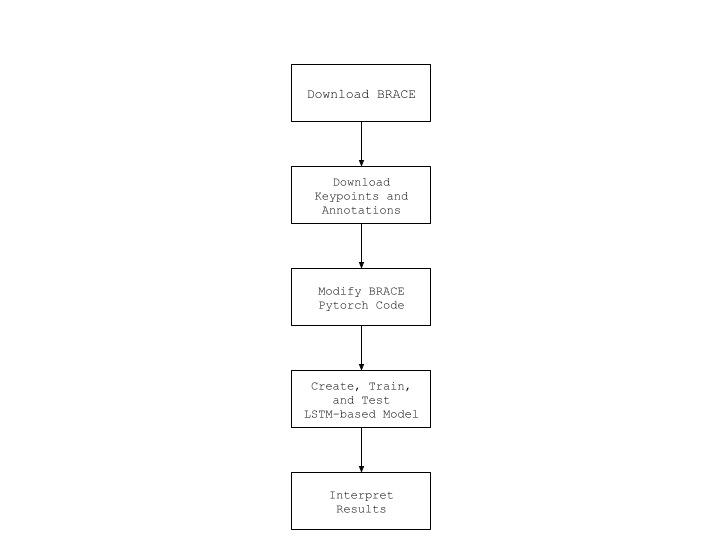
\includegraphics[width=\linewidth]{dpd.png}
    \caption{Development Process Diagram}
    \label{fig:1}
\end{figure}

\subsection{Dataset}
\par
Downloading BRACE has to be done manually in order to avoid copyright infringement. This is because the videos used in the dataset come from the Red Bull BC One channel on YouTube, so Red Bull owns the copyright to all the videos. The authors do however provide a guide in their Github repository, using the command line program \textit{youtube-dl} or \textit{ytdl} to download videos from YouTube from a terminal. The format to download videos is:

    \textit{youtube-dl -f 'bestvideo[ext=mp4]+bestaudio[ext=m4a]' [video ID]}


\subsection{Keypoints and Annotations}
\par
The BRACE Github repository \Textcite{brace} contains keypoints, audio features, and annotations of every sequence and segment in the BRACE dataset. Keypoints are sorted by year and by performance. They are further separated by genre where each file is a json file that splits the video into a genre performed by the dancer. Each file is a dictionary that contains an image file as the key which represents a single frame. Every frame has two values which are the bounding box and keypoints.

\subsection{Modifying the BRACE Pytorch Code}
\par To integrate the BRACE dataset into the PyTorch framework, Moltisanti's provided Python script from the same repository has been adapted. While originally designed to return sequences and metadata, the script has been modified to return sequence keypoints and their corresponding labels, specifically toprock, footwork, or powermove. The dataset can be instantiated by calling \textit{BraceDataset()}

\subsection{Creating, Training, and Testing the LSTM-based Model}
\par Figure 2 shows the Diagram of the LSTM-based model. 
\begin{figure}[htbp]
    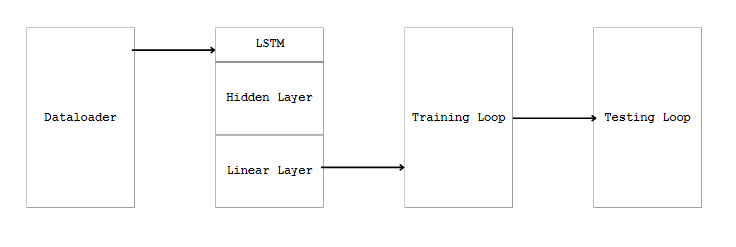
\includegraphics[width=\linewidth]{lstm flow.png}
    \caption{LSTM-based model diagram}
    \label{fig:2}
\end{figure}
\par The dataloader is divided into the training and testing splits, which were taken from the BraceDataset training and testing splits. PyTorch was the framework of use for this special probem, due to the PyTorch dataset already provided by \Textcite{brace}. 

\subsubsection{Hyperparameters, Loss Function, and Optimizer}
    \par The LSTM-based model employed the following hyperparameters, which have been tested to yield the highest accuracy possible.

    \begin{enumerate}
        \item Number of layers: 3
        \item Number of hidden layers: 2
        \item Learning rate: 0.01
        \item Batch size: 32
        \item Number of epochs: 15
    \end{enumerate}

    \par The loss function used for the model is Cross-Entropy Loss, which is ideal for classification tasks \parencite{CrossEntropy}. Furthermore, Adam was used as the optimizer of choice.

\subsection{Training and Testing}
\par The training process involved iterating over batches of data using a DataLoader, with each batch consisting of input sequences and their corresponding labels. The model's parameters were optimized using the Adam optimizer, with a learning rate of 0.01, and the CrossEntropyLoss function served as the criterion for evaluating the model's performance. During each epoch, the model iteratively updated its weights based on the computed loss, aiming to minimize the difference between predicted and actual labels.

\vspace{5mm}
\par For testing, the evaluation involved running the model on batches of testing data and calculating the test loss, as well as assessing the accuracy of the model's predictions. The model's performance was measured by comparing its predictions against the ground truth labels. It should be noted that the model was set to evaluation mode during testing, and the final accuracy, along with the test loss, was reported after completing the evaluation process. The achieved accuracy of 34.93\% suggests the current level of performance, which serves as a baseline for further model refinement and optimization in subsequent iterations.


\vspace{5mm}
\newpage
\section{Results and Discussion}
\subsection{Initial Results}
\par In the initial evaluation, the LSTM-based model yielded an accuracy of 34.93\%. This accuracy metric signifies the proportion of correct predictions made by the model among the total predictions. The achieved accuracy suggests that there is room for improvement in the model's performance for genre classification. Moving forward, it is recommended to delve deeper into analyzing if the instances that were misclassified to identify patterns or characteristics that can offer adjustments to the model architecture, hyperparameters, or data preprocessing steps. 
% LATEX table generator!!!!!!!!!!!!!
% gantt chart, this sem and next sem time frame
% implementation
% IMPLEMENTATION
% GANTT CHART
%download dataset
\newpage
\nocite{*}
\printbibliography
\newpage
\end{document}